%!TEX TS-program = xelatex
%!TEX encoding = UTF-8 Unicode

\documentclass[10pt]{article}
\usepackage[danish]{babel}


% fonts
\usepackage{fontspec,xltxtra,xunicode}
\defaultfontfeatures{Mapping=tex-text}
\setromanfont[Mapping=tex-text]{Adobe Garamond Pro}
\setsansfont[Scale=MatchLowercase,Mapping=tex-text]{Helvetica Neue}
\setmonofont[Scale=MatchLowercase]{Open Sans}
\renewcommand{\familydefault}{\sfdefault}


\usepackage{xcolor}
\definecolor{blue}{HTML}{1F497D}
\definecolor{warmgrey}{HTML}{F9F8F2}
\definecolor{darkblue}{RGB}{3,29,92}




% layout

\usepackage[showcrop, includehead, includefoot]{geometry}
\geometry{a4paper, layoutsize={168mm,237mm}, top=8mm, bottom=8mm}

\usepackage[parfill]{parskip}

\usepackage{titlesec}
\titleformat{\section}
  {\vspace{.8ex}%
   \rmfamily\Huge}
  {\thesection}{.5em}{}

\titleformat{\subsection}
	{\vspace{.2ex}%
	   \rmfamily\Large}
	{\thesubsection}{.5em}{}

\titleformat{\subsubsection}
	{\vspace{.2ex}%
	 \rmfamily\large}
	{\thesubsubsection}{.5em}{}

\usepackage{fancyhdr}
\pagestyle{fancy}

\renewcommand{\headrulewidth}{0.0pt}
\renewcommand{\footrulewidth}{0.2pt}
\lhead{\nouppercase{\rightmark}}
\chead{}
\rhead{}
\lfoot{\sffamily\small FDA 1.0 $\cdot$ Oktober 2017}
\cfoot{}
\rfoot{\sffamily\small \thepage}


%toc
\usepackage{tocloft}
\setcounter{tocdepth}{2}

% tt
\let\OldTexttt\texttt
\renewcommand{\texttt}[1]{\OldTexttt{\color{darkblue}{#1}}}

% figur
\usepackage{graphicx, grffile}
% set default figure placement to htbp
\makeatletter
\def\fps@figure{htbp}
\def\maxwidth{\ifdim\Gin@nat@width>\linewidth\linewidth\else\Gin@nat@width\fi}
\def\maxheight{\ifdim\Gin@nat@height>\textheight\textheight\else\Gin@nat@height\fi}
\makeatother
\setkeys{Gin}{width=\maxwidth,height=\maxheight,keepaspectratio}

\usepackage{mdframed} % colored backgrounds

\usepackage{floatrow}
%\floatsetup[figure]{style=plaintop}
\DeclareColorBox{shaded}{\colorbox{warmgrey}}
\floatsetup{style=plaintop,framestyle=colorbox,colorframeset=shaded,framefit=yes,heightadjust=all,framearound=all}


\usepackage{caption}
\DeclareCaptionFont{darkblue}{\color{darkblue}}
\captionsetup{
	font=small,
	format=plain,
	labelfont={darkblue,sf,up,bf},
	labelsep=newline,
	textfont={sf,up},
	justification=justified,
	singlelinecheck=false}




\usepackage{amsmath}
\numberwithin{figure}{section}


% styles
%\titlelabel{\llap{\thetitle\quad}} % numbers to the left

\setlength{\emergencystretch}{3em}  % prevent overfull lines

\usepackage[unicode=true]{hyperref}
\hypersetup{
            pdfborder={0 0 0},
            breaklinks=true}
\urlstyle{same}  % don't use monospace font for urls

\usepackage[normalem]{ulem}
% avoid problems with \sout in headers with hyperref:
\pdfstringdefDisableCommands{\renewcommand{\sout}{}}

\providecommand{\tightlist}{%
\setlength{\itemsep}{0pt}\setlength{\parskip}{0pt}}

\usepackage{enumitem}
\setlist[description]{font={\sffamily\mdseries\color{blue}}}

\usepackage{titlesec}
\newcommand{\sectionbreak}{\clearpage}
\renewcommand{\baselinestretch}{1.2}

%\setcounter{secnumdepth}{0} % numbers to what level

% use upquote if available, for straight quotes in verbatim environments
\IfFileExists{upquote.sty}{\usepackage{upquote}}{}
% use microtype if available
\IfFileExists{microtype.sty}{%
\usepackage[]{microtype}
\UseMicrotypeSet[protrusion]{basicmath} % disable protrusion for tt fonts
}{}
\PassOptionsToPackage{hyphens}{url} % url is loaded by hyperref





\title{\rmfamily\Huge Fællesoffentlig referencearkitektur \\ for deling af data og dokumenter}
\author{}
\date{\rmfamily Oktober 2017}

\begin{document}
\maketitle \clearpage

\tableofcontents
\newpage


\section*{Resume}\label{resume}

Hverdagen er digital, og data om borgere, virksomheder, myndigheder,
ejendomme, steder, køretøjer o.m.m. vedligeholdes i en lang række
områder af den offentlige administration. Der ligger et stort potentiale
i at gøre sådanne data tilgængelige for genbrug, så de kan skabe værdi i
andre sammenhænge end formålet med det oprindelige register. Dette kan
danne fundament for langt bedre understøttelse af tværgående, offentlige
services, og åbner tillige for anvendelse af data i nye og innovative
sammenhænge.

Men deling af data kan være teknisk kompliceret og i mange tilfælde
omkostningstungt, bl.a. drevet af krav til sikkerhed og dermed bevarelse
af borgeres og virksomheders tillid til datadeling i det offentlige
Danmark. Derfor er potentialet i deling og genbrug af data i høj grad
forblevet uindfriet.

Denne referencearkitekturs formål er at hjælpe med at indfri dette
potentiale. Dette gøres ved at introducere en fælles beskrivelse af de
begreber og sammenhænge, der er væsentlige for at forstå og arbejde med
design og implementering af løsninger, der involverer deling af data og
dokumenter. Dette sker både på det strategiske plan, hvor vision, mål og
arkitektoniske principper fastlægges; på det forretningsmæssige plan,
hvor de typiske brugsscenarier beskrives; og på det tekniske plan, hvor
en række implementeringsmønstre angiver, hvordan man i og mellem
applikationer kan dele og forsende data.

Referencearkitekturen er udarbejdet under den fællesoffentlige
digitaliseringsstrategi 2016-2020 og er som sådan relevant for alle
offentlige myndigheder og deres leverandører samt for virksomheder, der
ønsker at gøre brug af offentlige data.

\section{Introduktion}\label{introduktion}

\subsection{Formål og målgruppe}\label{formuxe5l-og-muxe5lgruppe}

Referencearkitekturen for deling af data og dokumenter understøtter
design, udvikling og anvendelse af offentlige it-systemer, der

\begin{itemize}
\tightlist
\item
  (gen)anvender oplysninger i form af data og dokumenter til
  sagsbehandling eller selvbetjening
\item
  sender eller modtager meddelelser fra andre it-systemer
\end{itemize}

Dokumentet er primært målrettet it-arkitekter tilknyttet offentlige
digitaliseringsprojekter, herunder enterprise-arkitekter,
forretningsarkitekter og løsningsarkitekter, der har til opgave at
kravspecificere og designe løsninger.

De første dele af dokumentet (Strategisk og Forretningsmæssig
arkitektur) henvender sig endvidere til projektledere og
beslutningstagere, herunder forretningsansvarlige,
digitaliseringschefer, it-chefer, afdelings- og kontorchefer og andre
med rollen som systemejer.

Dokumentet i sin helhed er også relevant for leverandører at orientere
sig i.

\subsection{Scope}\label{scope}

Referencearkitekturen beskriver anvendelse af og udvikling af
it-systemer, der reguleres af blandt andet:

\begin{description}
\tightlist
\item[EU databeskyttelse]
\emph{lov} som beskriver pligter og rettigheder ved behandling af
persondata
\item[EU eIDAS]
\emph{lov} som definerer registrede tillidstjenester
\item[Persondatalov]
\emph{lov} som beskriver pligter og rettigheder ved behandling af
persondata
\item[Lov om Digital Post]
\emph{lov} der gør det obligatorisk for virksomheder og borgere at
modtage digitale meddelelser fra offentlige afsendere.
\end{description}

Referencearkitekturen skrives på baggrund af den fællesoffentlige
digitaliseringsstrategi 2020 under initiativ 8.1 med tilslutning fra FM,
UFM, EVM, SIM, JM, EFKM, MBUL, SÆM, SKM, MFVM, BM, KL og Danske
Regioner. Heri beskrives referencearkitekturen således:

\begin{quote}
For at operationalisere, hvilke krav hvidbogen konkret stiller til
initiativer og systemer udarbejdes en referencearkitektur for deling af
data og dokumenter, der blandt andet beskriver fælles behovsmønstre og
mønstre for teknisk understøttelse, herunder de forskelige roller, der
skal afklares i initiativerne. Referencearkitekturen udpeger også
eventuelle områder for eksisterende og nye fælles standarder og
infrastruktur, som skal lette initiativernes implementering.
Referencearkitekturen bliver således en generel ramme og støtte for alle
initiativernes egen specifikke arkitektur.
\end{quote}

Uden for scope:

\begin{itemize}
\tightlist
\item
  åbne data, der ikke kræver adgangskontrol
\item
  registrering og anvendelse af data hos registerejer
\end{itemize}

\subsection{Centrale begreber}\label{centrale-begreber}

I det efterfølgende vil begrebet data blive brugt til at betegne både
oplysninger på dokumentform og oplysninger der optræder i registre. Vi
anvender begrebet datasamling både om et register og et repository med
dokumenter.

\begin{figure}
\centering
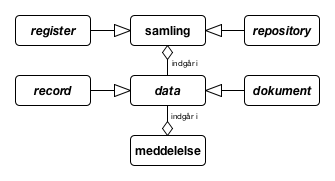
\includegraphics[width=\textwidth]{figures/abstraktion.png}
\caption{Anvendelse af begrebet data og relaterede begreber i denne
referencearkitektur}
\end{figure}

Vi vil endvidere lave en skelnen mellem:

\begin{itemize}
\tightlist
\item
  Anvendelse af udstillede data - typisk via API i
  system-til-system-integrationer
\item
  Forsendelse af meddelelser indeholdende data (herunder dokumenter) -
  typisk brugt ved beskeder til borgere/virksomheder, der skal have
  retsvirkning, men også et klassisk mønster brugt i
  system-til-system-integrationer.
\end{itemize}

Den fundamentale forskel på disse to scenarier er, om det er afsenderen
eller modtageren af data, der kender formålet med interaktionen. Ved
udstiling af data er dataafsenderen som udgangspunkt ikke bekendt med
datamodtagerens formål (men er naturligvis forpligtet til at håndhæve
relevant hjemmel). Ved forsendelse af meddelelser er det dataafsenderen,
der i en given kontekst afsender en meddelelse med et givent formål -
typisk som led i en proces.

\subsection{Anvendelse}\label{anvendelse}

Referencearkitekturen skal:

\begin{itemize}
\tightlist
\item
  danne et fælles sprog til at formulere en fælles handlingsplan
\item
  bruges som reference ved løsningsbeskrivelser
\end{itemize}

\subsection{Tilblivelse og governance}\label{tilblivelse-og-governance}

Første udgave er skrevet hos Kontor for Data og Arkitektur af Mads
Hjorth, Digitaliseringsstyrelsen og Anders Fausbøll, Omnium Improvement.

Endelig godkendelse forventes hos Styregruppe for Data og Arkitektur
under Digitaliseringsstrategien 18. december 2017.

\subsection{Metoderamme}\label{metoderamme}

Referencearkitekturen er udarbejdet inden for rammerne af
Fællesoffentlig Digital Arkitektur og følger så vidt muligt den fælles
skabelon for referencearkitekturer som udarbejdet i DIGST/KDA.
Metoderammen bygger blandt andet på erfaringer fra OIO
referencearkitektur, og indarbejder også elementer fra EIRA, TOGAF,
ArchiMate m.m.

Særlige elementer er i dokumentet angivet i \emph{kursiv} (fx
\emph{lov}, \emph{mål}, \emph{rolle} m.m.). Dette markerer, at de hører
til Archimate-begrebsapparatet.

\subsection{Relation til andre
referencearkitekturer}\label{relation-til-andre-referencearkitekturer}

Denne referencearkitektur gør brug af:

\begin{itemize}
\tightlist
\item
  Fællesoffentlig referencearkitektur for brugerstyring
\end{itemize}

Den skal kunne anvendes af:

\begin{itemize}
\tightlist
\item
  Fællesoffentlig referencearkitektur for selvbetjening
\item
  Fællesoffentlig referencearkitektur for overblik over egne sager og
  ydelser
\end{itemize}

\ldots{} og skal anvendes i kontekst sammen med:

\begin{itemize}
\tightlist
\item
  Deling af dokumenter på sundhedsområdet
\item
  Indberetning til registre på sundhedsområdet
\item
  Sag- og dokument på det kommunale område
\end{itemize}

\section{Strategisk arkitektur}\label{strategisk-arkitektur}

Udarbejdelsen af referencearkitekturen tager udgangspunkt i en række
identificerede forretningsmæssige og teknologiske trends og tendenser.

\subsection{Forretningsmæssige
tendenser}\label{forretningsmuxe6ssige-tendenser}

\begin{itemize}
\tightlist
\item
  Nationalt ønske om at undgå knopskudte løsninger
\item
  Data har øget værdi for organisationer
\item
  Øget bevågenhed omkring beskyttelse af privatliv
\item
  Øget opmærksomhed om håndtering af personlige oplysninger
\item
  Mængden af oplysninger der håndteres stiger
\item
  Grænseoverskridende services
\end{itemize}

\subsection{Teknologiske tendenser}\label{teknologiske-tendenser}

\begin{itemize}
\tightlist
\item
  øget central standardisering af begreber, datamodeller og grænseflader
\item
  Flere og mere forskelligartede enheder forbundet til netværket
\item
  Øgede forventninger til brugervenlighed af offentlige digitale
  services
\item
  Mængden af tilgængelige oplysninger vokser
\item
  Arkitekturvision for anvendelse og udstilling
\item
  Integrated Service Delivery
\item
  ''Interoperability/Samarbejdende infrastrukturer / Økosystem af fælles
  løsninger?''
\item
  ''Valgfrihed for anvender mellem flere tekniske udbydere af samme
  oplysninger''
\end{itemize}

\subsection{Strategiske
målsætninger}\label{strategiske-muxe5lsuxe6tninger}

De overordnede målsætninger for denne referencearkitektur kobler alle
til visionen om det datadrevne samfund, hvor data ses som et råstof for
samfundsudviklingen.

Målsætningerne inkluderer:

\begin{description}
\tightlist
\item[Interoperabilitet]
\emph{mål} om sammenhængende services\ldots{} integrated service
delivery
\item[Once-only]
\emph{mål} om at borger og virksomhed kun skal afgive den samme
information til det offentlige en gang\ldots{} (men give lov til
genbrug?)
\item[Transparens]
\emph{mål} om at borgere og virksomheder skal kunne se, hvilke data der
findes om dem, og hvor disse data anvendes
\item[Genbrug]
\emph{mål} om genbrug af it med henblik på lavere omkostninger
\end{description}

\subsection{Vision}\label{vision}

Visionen i denne referencearkitektur er at stræbe efter en situation,
hvor:

\begin{quote}
\emph{Data betragtes som en fælles, værdifuld og velbeskyttet ressource;
de skal være nemme at dele og bruge, men svære at misbruge}
\end{quote}

\begin{quote}
\emph{Data beskrives, fordeles, forbedres og beskyttes i fælleskab.}
\end{quote}

\begin{quote}
\emph{Fælles metoder for datadeling understøtter sammenstilling af data
og tværgående brug blandt myndigheder og virksomheder}
\end{quote}

\begin{quote}
\emph{Beskrivelse af, adgang til og brug af data sker under klar
governance og håndhæves ud fra tydelig hjemmel}
\end{quote}

\begin{quote}
\emph{Borgere og virksomheder har overblik over deres data og hvor, de
anvendes}
\end{quote}

\subsection{Værdiskabelse}\label{vuxe6rdiskabelse}

Værdien ved at følge denne referencearkitektur er, at den giver:

\begin{itemize}
\tightlist
\item
  Mindre besvær for borger og virksomheder ved brug af digitale services
\item
  Simplere arbejdsgange og mere potentiale for automatisering hos
  organisationer (myndigheder/virksomheder)
\item
  Understøttelse af værdiskabende innovation (ved at gøre data til et
  `råstof' for vækst/skabelse af konkurrencefordele)
\item
  Understøttelse transparens og bevare tillid til registre
\item
  Effektiv systemudvikling (begrænser udfaldsrum, opsamler best
  practice)
\end{itemize}

\subsection{Strategiske principper}\label{strategiske-principper}

Forretningsmæssige, Informationsmæssige, Applikationsmæssige og Tekniske
principper bag referencearkitekturen:

\begin{itemize}
\tightlist
\item
  F1: Byrden i datadeling skal afløftes fra dataejer, hvis den begrænser
  genbrug
\item
  F2: Autoritative registre med henvisninger til andre registre
\item
  F3: Ansvar for begrænsning af adgang ligger hos registerejer
\item
  I1: Fælles referenceinformationsmodel
\item
  I2: Dokument-princip (attester mv.)?
\item
  A1: Onlineopslag i sagsbehandling og selvbetjening
\item
  A2: Log adgang
\item
  A3: Adgang til og fra internationale registre sker gennem national
  gateway
\item
  T1: Central fuldmagts-/rettighedsstyring
\item
  T2: Multi-flavour-api
\end{itemize}

\section{Forretningsmæssig
arkitektur}\label{forretningsmuxe6ssig-arkitektur}

\subsection{Aktører}\label{aktuxf8rer}

De væsentligste aktører, der er i spil omkring deling af data og
dokumenter, er:

\begin{itemize}
\tightlist
\item
  Offentlige myndigheder, herunder virksomheder, der handler på vegne af
  offentlige myndigheder
\item
  Borgere og virksomheder
\end{itemize}

\subsection{Opgaver}\label{opgaver}

Forretningsmæssigt set finder referencearkitekturen anvendelse i
løsningen af alle offentlige opgaver. Specifikt kan nævnes:

\begin{itemize}
\tightlist
\item
  Borger- og virksomhedsvendte selvbetjeningsløsninger
\item
  Myndigheders sagsbehandling
\item
  Tværgående analyse, tilsyn og kontrol
\end{itemize}

\subsection{Funktioner}\label{funktioner}

Referencearkitekturen kredser om tre centrale use cases, hvor aktører
arbejder sammen i forskellige roller.

\begin{figure}
\centering
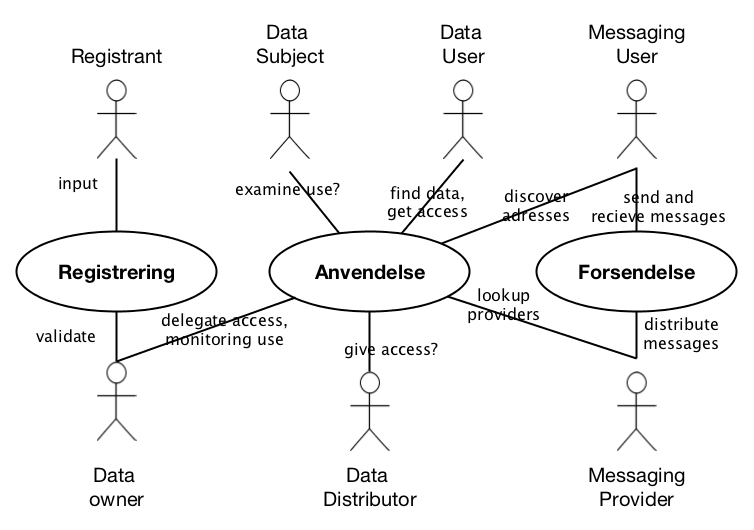
\includegraphics[width=\textwidth]{figures/usecases.png}
\caption{Tværgående use cases og funktioner hos de enkelte roller}
\end{figure}

De tre use cases er:

\begin{description}
\tightlist
\item[Registrering]
\emph{collaboration} hvor oplysninger bringes på digital form
\item[Anvendelse af udstillede data (herunder dokumenter)]
\emph{collaboration} hvor oplysninger anvendes i en opgave
\item[Forsendelse af meddelelser]
\emph{collaboration} hvor meddelelser sendes uafviseligt
\end{description}

\subsection{Roller}\label{roller}

I ovenstående use cases indgår disse roller:

\begin{description}
\tightlist
\item[Registrant]
\emph{rolle} som bringer oplysninger på digital form, registrer
\item[Datasubject]
\emph{rolle} som oplysninger handler
\item[Dataanvender]
\emph{rolle} der anvender oplysninger fra et register
\item[Dataejer]
\emph{rolle} som ejer registreringer/data, ansvar for at udarbejde
adgangspolitik
\item[Datadistributør]
\emph{rolle} som distribuerer data, ansvar for at håndhæve
adgangspolitik
\item[Messaging User]
\emph{rolle} som der sender og modtager meddelelser
\item[Messaging Provider]
\emph{rolle} som leverer services til forsendelse
\end{description}

Nogle af overnstående roller kan betragtes som specialiseringer af
GDPR-rollen \emph{Databehandler}.

\subsection{Use cases}\label{use-cases}

\begin{figure}
\centering
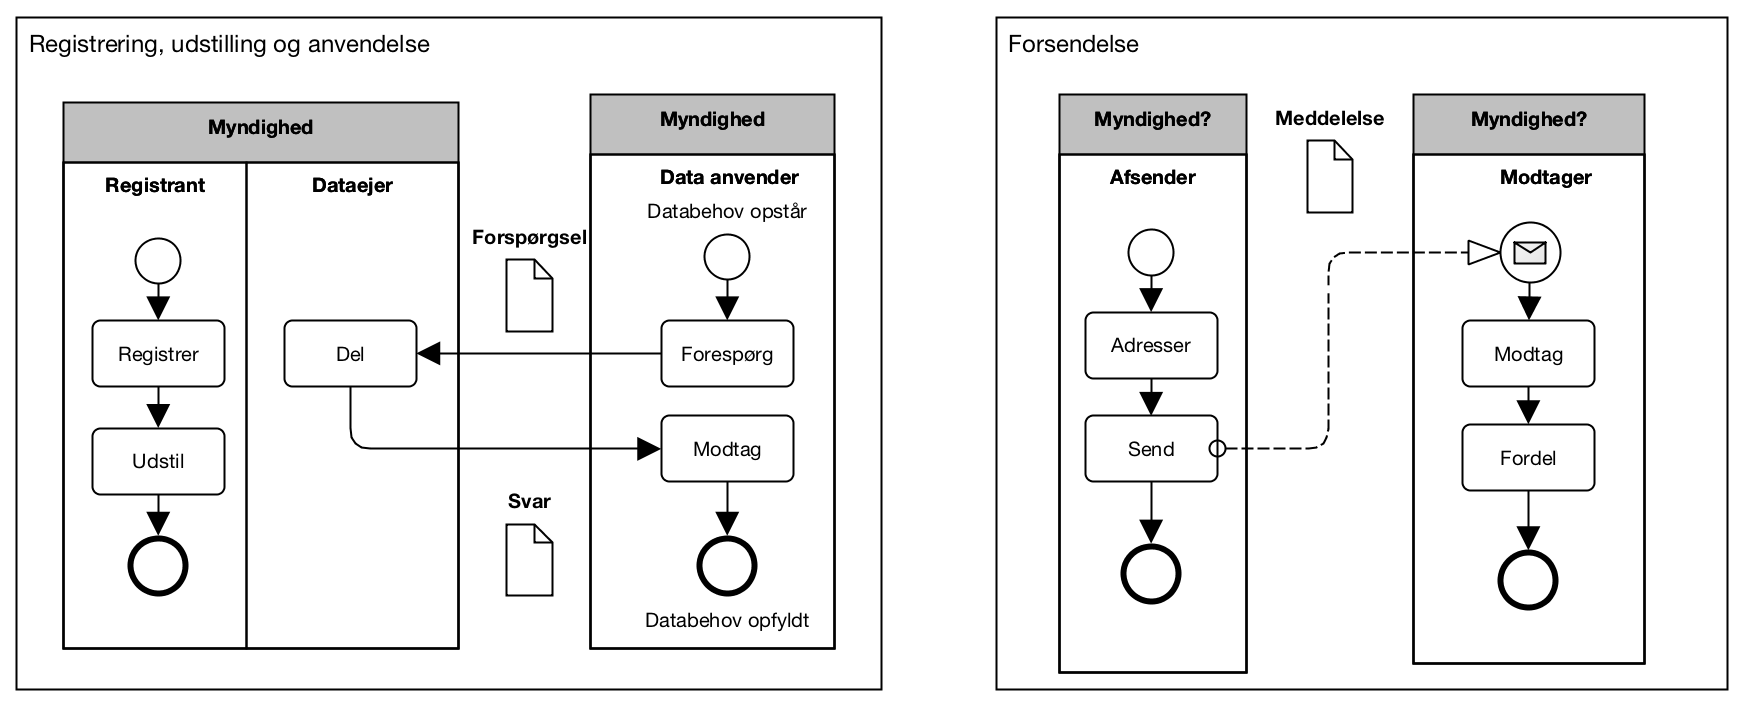
\includegraphics[width=\textwidth]{figures/patterns.png}
\caption{Overblik over centrale processer og deres aktiviteter fordelt
på roller}
\end{figure}

Figuren ovenfor beskriver det overordnede procesflow i de tre use cases.
Væsentligt at fremhæve er:

\begin{description}
\tightlist
\item[Registrering]
\emph{proces} En registrant initierer processen ved at registrere ny
data hos Dataejer (der er ansvarlig for sikring af hjemmel og
håndhævelse af adgangspolitik). Når data er korrekt registreret, skal
det markeres som klar til at blive udstillet.
\item[Anvendelse af udstillede data]
\emph{proces} Denne proces initieres hos Dataanvender - typisk en
myndighed, men kan også være en virksomhed - ud fra startsituationen, at
man har erkendt et behov for data. Dataanvender sender en forespørgsel
på data, der beskriver dels, hvilke data, der ønskes, og dels med
hvilken hjemmel. Dataejer håndhæver på denne baggrund adgangskontrol,
inden data deles og sendes i et svar til Dataanvender. Slutsituationen
bliver, at Dataanvenders databehov er opfyldt. Dataejer er ikke
nødvendigvis klar over, hvilket databehov forespørgslen har tjent til at
tilfredsstille - så længe, adgangen er legitim, kender Dataejer ikke
formålet med Dataanvenders brug af data.
\item[Forsendelse af meddelelser]
\emph{proces} Til forskel fra Anvendelse af udstillede data starter
denne proces hos Afsenderen (der tillige kan være Dataejer). Afsender
har udvalgt og pakketeret data i en Meddelelse (evt. i form af et
dokument), adresserer Meddelelsen og sender den herefter til Modtager.
Modtager kan være alle typer af aktører; i figuren er vist, hvordan det
hos en myndighed kan være relevant at fordele/route Meddelelsen internt
ud fra adresseringsoplysningerne. I sammenligning med Anvendelse af
udstillede data er det nu Afsender, der som deler af data `ejer' den
fulde forretningskontekst - hvor Dataejer overnfor ikke var bekendt med
formålet med at dele data.
\end{description}

\subsection{Tværgående processer}\label{tvuxe6rguxe5ende-processer}

Herunder beskrives, hvor de enkelte business functions hos de enkelte
roller anvendes i kontekst af et sæt af generiske procesmønstre.

\begin{itemize}
\tightlist
\item
  Sagsbehandling (fra Referencearkitektur for Sag og dokument)
\item
  Selvbetjening (fra Referencearkitektur for Selvbetjening)
\item
  Indsigt i oplysninger og deres anvendelse (fra Referencearkitektur for
  Overblik over sag og ydelser)
\item
  Sende meddelelse (inkl. brug af tilmeldingslister og påmindelser)
\item
  Modtage meddelelse
\item
  Tag et dokument med til en anden service provider, der ikke har adgang
  til registre - herunder beskrive, hvordan dokumenter valideres.
\end{itemize}

\subsection{Forretningstjenester}\label{forretningstjenester}

Procestrin udtrykkes typisk ved Forretningstjenester, der igen kan
realiseres af interne business functions eller trække på eksterne
business services.

\subsection{Forretningsobjekter}\label{forretningsobjekter}

Nedenfor fremgår en initiel oversigt over en række forretningsobjekter,
der er væsentlige for referencearkitekturen. Det videre arbejde skal
klarlægge, hvilke elementer der skal indgå i listen samt hvordan de
defineres. Modelleringsniveauet skal endvidere lægges fast
(begrebsmodellering og/eller logiske kernemodeller?)
Kommentarer/regibemærkninger indgår i listen, markeret med kantede
parenteser.

\begin{figure}
\centering
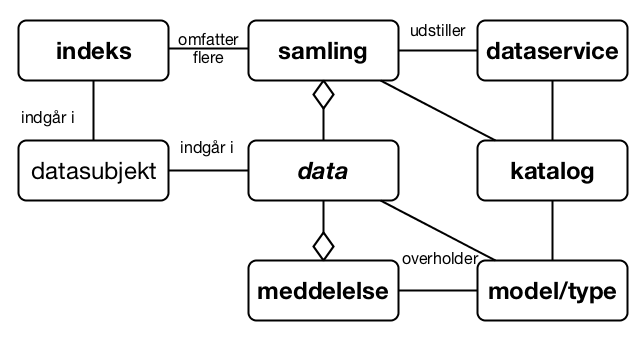
\includegraphics[width=\textwidth]{figures/objekter.png}
\caption{Oversigt over de centrale forretningsobjekter og deres
relationer}
\end{figure}

\begin{description}
\tightlist
\item[data]
\emph{objekt} (Abstrakt. Bruges om både registerrecord og dokument)
\item[samling]
\emph{objekt} {[}Datasætmodel har ikke definition\ldots{}{]} ISO9115: en
identificerbar samling af oplysninger (samlebetegnelse for PSI, GPDR, )
\item[meddelelse]
\emph{objekt} {[}NgDP{]} registreret forsendelse
\item[datasubjekt]
\emph{objekt} {[}Grunddata, fx person. GPDR den registrede{]}
\item[model/type]
\emph{objekt} {[}Jf. modelregler fra FDA{]}
\item[katalog]
\emph{objekt} {[}jf hvidbog{]} både data, service\ldots{} til design
\item[dataservice]
\emph{objekt} webservice med adgang til datasamling
\end{description}

og andre mulige

\begin{description}
\tightlist
\item[registeroplysning]
\emph{objekt} en record
\item[dokument]
\emph{objekt} {[}Dokumentmodel fra OIO{]}
\item[påmindelse]
\emph{objekt} {[}Næste generation Digital Post{]}
\item[registreringshændelse]
\emph{objekt}
\item[forretningshændelse]
\emph{objekt}
\item[klassifikation]
\emph{objekt}
\end{description}

\subsection{Forretningsmønstre}\label{forretningsmuxf8nstre}

\emph{TBU.}

\section{Teknisk arkitektur}\label{teknisk-arkitektur}

Dette afsnit beskriver roller og implementeringsmønstre, der er
relevante, når forretningsfunktionerne beskrevet ovenfor skal
understøttes/realiseres af applikationer. Endvidere udpeges områder, der
er kandidat til standardisering og/eller profilering i forbindelse med
referencearkitekturen.

De nødvendige og understøttende applikations-services og deres indbyrdes
relationer er vist i figuren nedenfor.

\begin{figure}
\centering

\includegraphics[width=\textwidth]{figures/services.png}
\caption{Oversigt over nødvendige og understøttende
applikations-services og deres indbyrdes relationer}
\end{figure}

\subsection{Applikationsroller}\label{applikationsroller}

\begin{description}
\tightlist
\item[eDelivery Service Provider]
\emph{applikationsservice} som skal kunne:
\end{description}

\begin{itemize}
\tightlist
\item
  udstille eller levere meddelelser til modtager
\item
  modtage og distribuere meddeleleser
\item
  fortælle andre om deres kunder
\end{itemize}

\begin{description}
\tightlist
\item[Dataservice]
\emph{applikationsservice} som skal kunne:
\end{description}

\begin{itemize}
\tightlist
\item
  opbevare datasamling
\item
  begrænse adgang til de rigtige
\item
  (måske) vedligeholde og udsende abonnementer MBK:
\end{itemize}

\begin{description}
\tightlist
\item[Kontaktregister]
\emph{applikationsservice} som er en slags data service med en særlig
type oplysninger
\item[Log]
\emph{applikationsservice} som er en slags data service med særlige
oplysninger
\item[Indeks]
\emph{applikationsservice} som er en slags data service med særlige
oplysninger. Kan undværes, men på kraftig bekostning af effektivitet i
bestemte situationer.
\item[Katalog]
\emph{applikationsservice} som ikke er en dataservice, fordi der ikke er
begrænset adgang. Kan undværes, men ikke effektivt.
\end{description}

\subsection{Tekniske Implementeringer}\label{tekniske-implementeringer}

Her grupperes de enkelte roller og applikationsroller jf. forskellige
mønstre.

\subsubsection{Anvendelse af udstillede
data}\label{anvendelse-af-udstillede-data}

Når en dataanvender (virksomhed eller myndighed) vil have adgang til
data hos en dataejende myndighed, kan det ske via ét af nedenstående tre
mønstre: {[}TODO: Overvej samtykker ift. Virksomhed\textgreater{}{]}: x
{[}TODO: Overvej Hændelser\textgreater{}{]}: x

\paragraph{Direkte adgang}\label{direkte-adgang}

\begin{figure}
\centering

\includegraphics[width=\textwidth]{figures/use-soa.png}
\caption{Implementeringsmønster med direkte adgang til registre}
\end{figure}

I dette mønster, som er simpelt og måske det mest klassiske, er det
Dataejer, der selv udstiller data til de mulige anvendere via en
service-orienteret arkitektur. Dataejer er også ansvarlig for at betjene
Datasubjektets forespørgsler om Dataejerens brug af personlige data.

Fordelen ved dette mønster er, at det er simpelt. Ulempen er, at
Dataejer kommer til at bære hele udgiften ved at stille data bredt til
rådighed.

\paragraph{Datadistribution}\label{datadistribution}

\begin{figure}
\centering
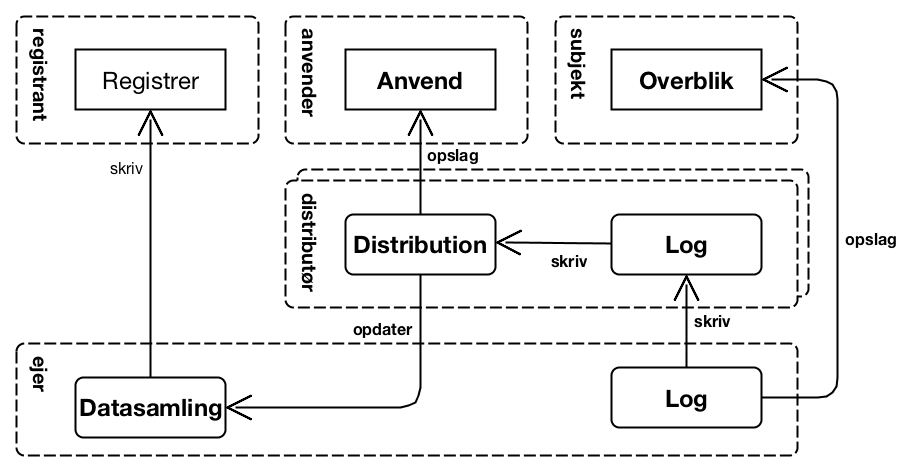
\includegraphics[width=\textwidth]{figures/use-dist.png}
\caption{Implementeringsmønster for datadistribution}
\end{figure}

I dette mønster er Dataejer fortsat ansvarlig for registrering af data.
Anvendelsesdelen er imidlertid afløftet til en Datadistributør (evt.
flere). Dette giver Datadistributøren mulighed for at fokusere netop på
distributionen, dvs. at gøre data bredt tilgængeligt (dog naturligvis
under håndhævelse af adgangskrav specificeret af Dataejer) til
Dataanvendere.

Når nye data registreres, er Dataejer ansvarlig for at opdatere
Datasamlingen hos Datadistributøren.

Logningsmæssigt er den enkelte Datadistributør ansvarlig for at logge
Dataanvenders adgang til data. Samtidig er den enkelte Distributør
ansvarlig for at sørge for konsolidering af loggen. I figuren er
log-konsolidering lagt hos Dataejer, men den kunne i princippet også
være uddelegeret - så længe, der er et entydigt og klart SPOC for
Datasubjektets opslag i anvendelsen af personlige data.

\paragraph{Distribueret service- og
data-platform}\label{distribueret-service--og-data-platform}

\begin{figure}
\centering
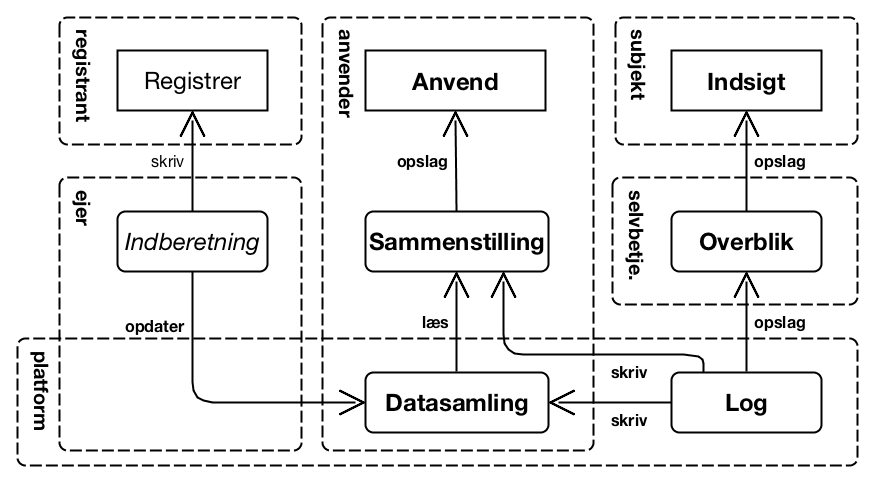
\includegraphics[width=\textwidth]{figures/use-plat.png}
\caption{Implementeringsmønster for distribueret dataplatform}
\end{figure}

Delingsansvaret er i dette mønster i høj grad håndteret af en
Dataplatform. Platformen er distribueret og er i stand til at replikere
data på tværs af Dataejer og Dataanvendere. Dvs., at data, der
registreres via Dataejer, gøres tilgængelige hos Dataanvender af
platformen.

Da Dataplatformen kan rumme data fra forskellige Dataejere, muliggøres
effektiv sammenstiling af data hos Datanvenderen. Platformen er
ansvarlig for at håndhæve adgangskontrol, og eventuelle services hos
Dataanvender, der gør brug af data, er ansvarlige for at logge deres
brug. Platformen konsoliderer brugs-loggen, og gør det muligt for
Datasubjekt at få overblik over brug af personlige data.

Fordelen ved dette mønster er den umiddelbare og standardiserede
tilgænglighed til data, som en Dataplatform kan levere. Ulempen er, at
kompleksiteten øges, samt at der stilles større krav til Datanvenders
modenhed ift. den tekniske adgang til data (da Dataanvenders
applikationer i praksis vil skulle afvikles på den distribuerede
Service- og Dataplatform).

\emph{(Uafklaret: Skal Dataanvenders applikationer/services have direkte
adgang til distribuerede data, eller skal adgang fortsat ske via et
servicesnit, der kan varetage adgangskontol m.m.?)}

\subsubsection{Forsendelse af
meddelelse}\label{forsendelse-af-meddelelse}

Når en myndighed vil initiere en specifik og målrettet datadeling - dvs.
sende data (herunder dokumenter) til en anden myndighed, virksomhed
eller borger - kan det ske via ét af de tre nedenstående mønstre.

\paragraph{Sikker e-mail}\label{sikker-e-mail}

\begin{figure}
\centering
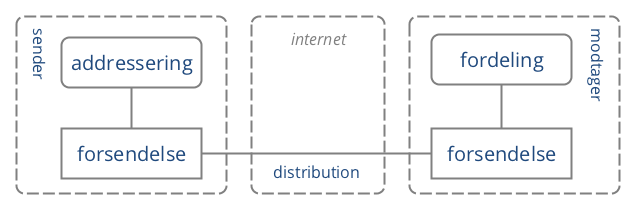
\includegraphics[width=\textwidth]{figures/send-email.png}
\caption{Implementeringsmønster for e-mail}
\end{figure}

Et meget anvendt mønster for myndighed til myndighed-kommunikation er at
levere en Meddelelse fra Afsender til Modtager ved brug af sikker
e-mail. Det falder uden for dette dokuments scope at beskrive dette
mønster yderligere, men det er medtaget her for reference. Det er
endvidere oplagt at betragte dette mønster som et særtilfælde af det
generelle `Service provider'-mønster nedenfor.

Fordelen ved dette mønster er, at det er simpelt og benytter sig af
standardteknologi. Ulempen er, at det kun dækker myndighed til
myndighed-kommunikation. Derudover sætter standardteknologien (e-mail)
visse begrænsninger for funktionalitet, der fx understøtter automatisk
routing af beskeder hos modtageren i det tilfælde, hvor Meddelelsen ikke
har én specifik modtager.

\paragraph{Fælles system}\label{fuxe6lles-system}

\begin{figure}
\centering
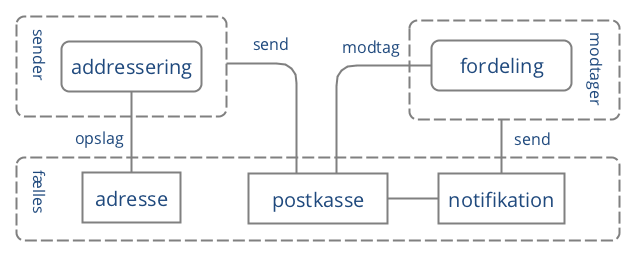
\includegraphics[width=\textwidth]{figures/send-shared.png}
\caption{Implementeringsmønster for fælles applikation}
\end{figure}

Ved brug af Fælles system-mønsteret til Forsendelse af en Meddelelse
benytter Afsender og Modtager et centralt, fælles system til hhv. at
placere Meddelelsen og læse den. I den analoge verden svarer dette
mønster til, at Afsender og Modtager benytter et fælles postbokskontor.
Digitalt er dette mønster fx implementeret af e-Boks, hvor såvel
myndigheder, virksomheder og borgere kan placere Meddelelser, der
efterfølgende kan hentes af Modtager. Også messaging-funktionaliteten i
mange af de sociale medieplatforme (fx Facebook) falder i denne
kategori.

TIl forskel fra Sikker e-mail-mønsteret ovenfor er Fælles
system-mønsteret mere robust, både da Forsendelsesservicen tilbyder
opslag/verifikation mod et Kontaktregister samt da Meddelelsen opbevares
i infrastrukturen, indtil Modtager aktivt læser den - i modsætning til
Sikker e-mail, hvori infrastrukturen blot videresender Meddelelsen og
dermed er afhængig af, at Modtageren i praksis findes.

Meddelelsesfunktionaliteten har endvidere mulighed for at trække på en
Notifikationsservice, der kan tilbyde notifikationer til Modtager om den
nye Meddelelse.

Et Fælles system-mønster kan fungere på mange niveauer, herunder
nationalt (fx Digital Post); inden for et specifikt domæne, fx på
sundhedsområdet; eller rent bilateralt, hvor to organisationer vælger en
Meddelelsesplatform og enes om dette mønster.

\paragraph{Økosystem/Service
providers}\label{uxf8kosystemservice-providers}

\begin{figure}
\centering
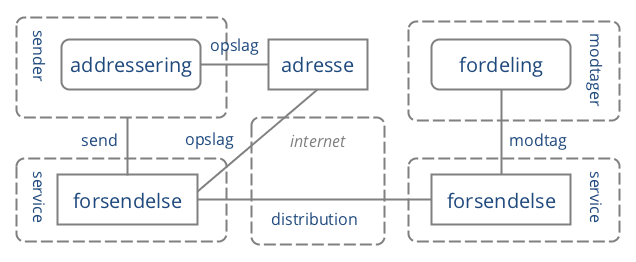
\includegraphics[width=\textwidth]{figures/send-eco.png}
\caption{Implementeringsmønster for ecosystem}
\end{figure}

I dette mønster deltager både Afsender (A) og Modtager (D) i et
Meddelelses-økosystem ved at vælge hver sin Forsendelses-Service
provider (hhv. B og C). Økosystem-mønsteret er bl.a. kendt i kontekst af
den europæiske eDelivery-standard som en \emph{four corner model}.

Et fælles Kontaktregister udgør en central komponent i økosystemet, der
gør det muligt for alle parter at slå den relevante information op. En
Afsender kan via Kontaktregisteret se/verificere mulige modtagere, samt
evt. afgøre hvilken konkrete Meddelelsesformater/kanaler, Modtager kan
håndtere. Forsendelsesservicen, der håndterer afsendelse af Meddelelsen,
kan benytte Kontaktregisteret til at finde Modtagerens konkrete Service
provider og bliver dermed i stand til at levere Meddelelsen.

Mønsteret vil typisk være symmetrisk, således at en Afsender også kan
indgå som Modtager og vice versa. Mønsteret kan i øvrigt både være
generisk eller specifikt for et domæne, der fx kan stille ekstra krav
til Meddelelsens format.

Fordelene ved Økosystem-mønsteret er, at det er robust, fleksibelt og
løbende kan udvides med nye Service providers. Ulempen er, at der
stilles store krav til det centrale Kontaktregister, samt at der fortsat
ikke findes standardteknologier, der dækker mønsteret.

\subsubsection{Registrering}\label{registrering}

Registrering af data er ikke i scope for denne referencearkitektur, men
medtages kort pga. sin væsentlige relation til Index-konceptet.

{[}TODO: Hvor udfolder vi mere om mønstre, der anvender Index?{]}

\begin{description}
\tightlist
\item[Ansvar hos registrant]
\emph{implementationsmønster}
\item[Ansvar hos dataejer]
\emph{implementationsmønster}
\item[Ansvar hos distributør]
\emph{implementationsmønster}
\end{description}

\subsection{Områder for
standardisering/profileringer}\label{omruxe5der-for-standardiseringprofileringer}

Nedenstående, tekniske områder er kandidater til at indgå i
referencearkitekturen i forhold til at pege på en anbefalet standard
eller en særlig profilering, evt. vendt mod de enkelte, tekniske
mønstre.

\begin{itemize}
\tightlist
\item
  Service Design Guidelines
\item
  Access Protocols
\item
  Distribution Protocols
\item
  Synchronisation Protocols
\item
  Metadata for opslag/søgning/anvendelse
\item
  Log format
\item
  Identifikation
\item
  Klassifikation af følsomhed
\item
  Klassifikation af anvendelse (sagsbehandling vs analyse)
\item
  Hændelsesbeskeder
\item
  Protokol for flytning af filer, kryptering
\item
  Hjemmel (samtykke, lov)
\item
  Context
\end{itemize}

\subsection{Identifikation af eksisterende
standarder}\label{identifikation-af-eksisterende-standarder}

\emph{TBU.}



\newpage
\thispagestyle{empty}
\begin{figure}
\includegraphics[angle=90, height=\textheight]{../overview.pdf}
\caption{Overblik over elementer i referencearkitekturen og deres EIRA stereotyper}
\end{figure}

\newpage
\thispagestyle{empty}
\begin{figure}
\caption{Overblik over elementer i de samlede referencearkitekturer i FDA}
\includegraphics[angle=0, width=\textwidth]{../eco2.pdf}

\end{figure}

\end{document}
